\documentclass[journal]{IEEEtran}
\usepackage{amsmath,amssymb}
\usepackage{graphicx}
\usepackage{array}
\usepackage{cite}
\usepackage{xcolor}
\newcommand{\rev}[1]{{\color{blue}#1}}
\newcommand{\new}[1]{{\color{red}#1}}
% --- Algorithms ---
\usepackage{algorithm}
\usepackage{algpseudocode}   % recommended (clean, modern)

% --- Math ---
\usepackage{amsmath,amssymb}

% --- Floats & formatting (optional but common) ---
\usepackage{float}           % for [H] placement if needed
\usepackage[caption=false,font=footnotesize]{subfig}

\usepackage{svg}

% --- Reviewer-requested references for CUSUM and EWMA ---
\begin{filecontents*}{reviewer_added_refs.bib}
@article{Page1954CUSUM,
  author  = {E. S. Page},
  title   = {Continuous Inspection Schemes},
  journal = {Biometrika},
  volume  = {41},
  number  = {1/2},
  pages   = {100--115},
  year    = {1954}
}
@article{Roberts1959EWMA,
  author  = {S. W. Roberts},
  title   = {Control Chart Tests Based on Geometric Moving Averages},
  journal = {Technometrics},
  volume  = {1},
  number  = {3},
  pages   = {239--250},
  year    = {1959}
}
@article{hyndman2006mape,
  author  = {R. J. Hyndman and A. B. Koehler},
  title   = {Another Look at Measures of Forecast Accuracy},
  journal = {International Journal of Forecasting},
  volume  = {22},
  number  = {4},
  pages   = {679--688},
  year    = {2006}
}
@article{Khorov2019Tutorial,
  author  = {E. Khorov and A. Lyakhov and A. Krotov and A. Guschin},
  title   = {A Tutorial on IEEE 802.11ah: A Wireless LAN for Internet of Things},
  journal = {IEEE Communications Surveys \& Tutorials},
  volume  = {21},
  number  = {2},
  pages   = {1738--1767},
  year    = {2019}
}
\end{filecontents*}


\title{Autonomous Predictive Traffic-Aware RAW Slot Sizing in IEEE 802.11ah-based IoT Networks}
\author{Alakesh~Kalita, ~\IEEEmembership{Senior Member,~IEEE}, and Nurzaman ~Ahmed,~\IEEEmembership{Member,~IEEE},
		% <-this % stops a space
		\thanks{ Manuscript received January X, 202X; revised December X, 202x; accepted February X, 202X. %The authors received partial financial support from SERB, India, for building the research testbed used in this article.
        \textit{(Corresponding author: Alakesh Kalita.)}}
		\IEEEcompsocitemizethanks{\IEEEcompsocthanksitem A. Kalita is with the Department of  Mathematics and Computing, Indian Institute of Technology (ISM) Dhanbad, India. \protect\\
		E-mail: alakesh.kalita1025@gmail.com\\
			N. \rev{Ahmed} is with Donald Danforth Plant Science Center, USA. \protect\\
		E-mail: nurzaman713@gmail.com

		}
	}
\begin{document}
\maketitle

\begin{abstract}
This paper presents a simple, standard-compliant, and adaptive mechanism for sizing Restricted Access Window (RAW) slots for the IEEE 802.11ah RAW-based channel access scheme in large-scale Internet of Things (IoT) networks. At first, in our proposed scheme, the Access Point (AP) autonomously predicts the packet demand per station (STA), i.e., without any control packet overhead or explicit information from the STAs. \rev{The AP combines CUSUM-based burst detection with EWMA-based demand tracking, estimates the active contenders in each RAW slot from local reception history, and maps the required service time to the RAW Parameter Set (RPS) slot-duration field under the available RAW airtime budget.} Based on the predicted number of packets per STA within a group and the number of contending STAs per RAW slot, we derive the RAW slot size in terms of backoff-slot units for the given group. %We propose another scheme to find adaptive upper and lower bound of RAW slot.
Experimental results, benchmarked against static allocation and two recent adaptive schemes (LACA, Chang2019), show that the proposed adaptive slot sizing significantly improves overall network throughput and packet delivery ratio compared to all three baselines\new{, achieving up to $2\times$ higher packet delivery ratio and throughput than static allocation and up to $9\times$ higher energy efficiency (bits delivered per joule) than the least efficient baseline, with the largest gains under low-to-moderate contention}. \rev{The scheme introduces no extra control packet and remains compatible with beacon-based IEEE~802.11ah RAW configuration.}
\end{abstract}

\begin{IEEEkeywords}
Internet of Things (IoT), IEEE 802.11ah, WiFi HaLow, Restricted Access Window, Adaptive slot sizing.
\end{IEEEkeywords}

\section{Introduction}

The IEEE~802.11ah standard \cite{IEEE80211ah2016} is specifically designed to support large-scale Internet of Things (IoT) networks comprising a massive number of low-power stations (STAs). To enable scalable channel access in dense networks, IEEE~802.11ah introduces a channel access mechanism based on the Restricted Access Window (RAW). RAW divides the beacon interval into multiple equal duration slots and allows some of the STAs to contend for transmission within a slot. The number of contenders in a slot solely depends on the Association IDs (AIDs) of the STAs, and by limiting the number of contenders, RAW significantly reduces channel congestion.

The Access Point (AP) announces RAW configuration parameters through the RAW Parameter Set (RPS) field embedded in beacon frames. Stations are hierarchically organized across Delivery Traffic Indication Map (DTIM) intervals, TIM periods, and RAW slots. Within a TIM period, one or more RAW segments may be defined, each further partitioned into multiple slots. A STA wakes up to receive its corresponding TIM beacon and is allowed to perform uplink or downlink communication only during its assigned RAW slot. Therefore, the efficiency of the RAW mechanism heavily depends on proper slot configuration and allocation \cite{IEEE80211ah2016, TIAN2021103036}.

% \begin{figure}[!h]
% 	\centering
% 	\includegraphics[width=\columnwidth]{RAW_slot.png}
% 	%\includegraphics[scale=0.4]{image/markov-states.pdf}
% 	\caption{Slot operation within a RAW group.}
% 	\label{raw_slot}
% \end{figure}

The RPS information element specifies the number of slots, slot format, and slot duration count sub-fields, which together determine the RAW slot duration as
\begin{equation}
D = 500~\mu s + C \times 120~\mu s,
\end{equation}
where $C$ is the slot duration count sub-field. %The length of $C$ is either 11 bits or 8 bits depending on the slot format field (set to 1 or 0, respectively).
%When the slot format is set to 1 (11-bit $C$), a RAW can contain at most 8 slots, and $C$ can take a maximum value of $2^{11}-1 = 2047$, resulting in a maximum slot duration of approximately 246.14~ms. When the slot format is set to 0 (8-bit $C$), a RAW can contain up to 64 slots, and $C$ can take a maximum value of $2^{8}-1 = 255$, limiting the maximum slot duration to approximately 31.1~ms.
Stations are mapped to RAW slots according to
\begin{equation}
i_{\text{slot}} = (x + N_{\text{offset}}) \bmod N_{\text{RAW}},
\end{equation}
where $N_{\text{RAW}}$ is the number of slots within a RAW, $N_{\text{offset}}$ is derived from the two least significant octets of the beacon Frame Check Sequence (FCS) to enhance fairness, and $x$ is either the station's index among active stations or its AID.

Since the slot assignment is based on a modulo operation over $N_{\text{RAW}}$, multiple stations may be mapped to the same slot, particularly when the total number of associated STAs exceeds the number of available RAW slots. %Consequently, a large number of STAs can contend simultaneously within a single RAW slot, leading to increased collision probability and higher access delay. Therefore, appropriate RAW slot sizing and grouping are critical for controlling contention in dense IEEE~802.11ah networks.
Consequently, in uplink communication, STAs contend for channel access using the standard contention-based procedure within their allocated RAW slot. As the number of contending STAs increases, collision probability rises, resulting in repeated \texttt{backoffs} and increased access delay. If the RAW slot duration is too small, excessive collisions and packet drops may occur. Conversely, oversized RAW slots lead to underutilized airtime and \rev{reduced overall efficiency in terms of packet latency and throughput}. Hence, accurate RAW slot sizing is critical to balancing contention, delay, and channel utilization. %However, even within a group, the number of contending stations per slot can remain high, making efficient channel utilization a challenging task.

Notably, numerous schemes exist to improve the performance of IEEE 802.11ah networks in various ways, such as traffic scheduling \cite{9037271}, TWT-Scheduling \cite{Busacca2026TWT},  MAC-enhancement \cite{9512279}, dynamic group management \cite{Chang2019TrafficAware}, and many more \cite{TIAN2021103036, 9512279}. %However, none of the existing works address the need for adaptive RAW slot sizing in large-scale IEEE 802.11ah networks.
The work in \cite{10067238} provided a solution for adaptive slot duration, but it is limited to analytical analysis and considers only a small number of nodes for evaluation. Again, the proposed solution in \cite{11165035} is not feasible for resource-constrained IEEE 802.11ah-supported boards.
Therefore, in this work, we \rev{propose} a scheme to make the RAW slot size adaptive depending on the number of active transmitting STAs and their traffic demand. %By doing this, contention and so collisions can be reduced, and channel utilization improved, all while maintaining full compliance with the IEEE~802.11ah MAC framework.
In brief, the major contributions of this work are as follows.
\begin{itemize}
    \item We autonomously predict the traffic of each STA without any control packet overhead or explicit information from the STAs. The proposed traffic prediction model achieves high accuracy and responds quickly to bursty traffic, \rev{as quantified using MAE, RMSE, and MAPE in the revised evaluation}.

    \item Based on the predicted traffic and the number of contending nodes, we develop a mathematical model that enables the AP to determine the appropriate RAW slot size for each group. To the best of our knowledge, this is the first work to derive a closed-form, standard-compliant RAW slot sizing rule directly in backoff-slot units using autonomous per-STA traffic prediction without control signaling overhead. \rev{We further analyze the AP-side computational complexity and scalability of the proposed CUSUM--EWMA update.}


    \item We perform extensive simulation by varying different network parameters. Simulation results show that our proposed adaptive slot mechansim provides better packet delivery \rev{ratio} (PDR), throughput\rev{,} and delay compared to the default static setting defined in IEEE 802.11ah standard.
\end{itemize}



\section{Proposed Autonomous RAW Slot Sizing Scheme}
Accurate RAW slot sizing requires reliable estimation of traffic demand within each RAW group, especially under dynamic and bursty conditions in IEEE~802.11ah networks. To avoid additional signaling overhead, in our proposed scheme, the AP autonomously estimates the packet demand of each STA based on locally observed transmissions and adapts the RAW slot duration accordingly. The following subsections describe the traffic estimation method and the corresponding RAW slot sizing mechanism.

\begingroup\color{blue}
Unless explicitly stated otherwise, the term \emph{RAW slot} is used for the time interval assigned by the RAW configuration, whereas \emph{backoff slot} or \emph{virtual slot} refers to the PHY/MAC contention time unit used inside a RAW slot. This distinction is maintained throughout the revised formulation to avoid ambiguity between RAW scheduling slots and DCF backoff slots.
\endgroup

\subsection{Traffic Load Estimation}

Consider an uplink between a child node $C$ and its parent (AP) $P$, where $C$ transmits and $P$ receives. Since RAW slot allocation is decided at the parent, $P$ must estimate the child\^{a}s traffic demand without explicit signaling. The estimation relies solely on locally observable receptions.

At the \rev{reception-slot} level, the parent estimates the transmission attempt rate using EWMA (Exponentially Weighted Moving Average) \rev{\cite{Roberts1959EWMA}}. Let $\hat{a}_{i,r}$ denote the estimated attempt rate at the $i$-th reception slot. \rev{Here, $r$ indexes the reception opportunity observed by the AP for STA $i$, and $\hat{a}_{i,r}$ represents the AP's smoothed estimate of whether STA $i$ is actively attempting uplink transmission. A reception slot is classified as \emph{Idle} if no energy or preamble is detected, \emph{Others} if a frame from another STA is decoded, \emph{Success} if a frame from STA $i$ is decoded, \emph{Collision} if overlapping transmissions prevent decoding, and \emph{Unavailable} if the AP cannot observe the slot because of scheduling or channel occupation.} The estimate is updated as
\begin{equation}
\hat{a}_{i,r} =
\begin{cases}
(1-\lambda)\hat{a}_{i-1,r}, & \text{No Tx (Idle or Others)} \\[4pt]
(1-\lambda)\hat{a}_{i-1,r} + \lambda, & \text{Tx (Success)} \\[4pt]
\hat{a}_{i-1,r}, & \text{Collision or Unavailable}
\end{cases}
\label{eq:attempt_ewma}
\end{equation}
where $\lambda \in (0,1)$ controls the tradeoff between stability and responsiveness.

At the interval level, let $D_t$ denote the number of packets received in scheduling interval $t$, and let $\mu_t$ be the estimated mean demand before observing $D_t$. The deviation is defined as $z_t = D_t - \mu_t$. To detect bursty traffic, we maintain a one-sided CUSUM (CUmulative SUM) statistic \rev{\cite{Page1954CUSUM}} as follows,
\begin{equation}
S_{t+1} = \max\{0,\, S_t + z_t - \kappa\}, \qquad S_0 = 0,
\label{eq:cusum_update}
\end{equation}
where $\kappa$ is a drift parameter used to avoid false burst indications due to small random fluctuations. If $S_{t+1}$ exceeds a threshold $H$, a traffic burst is declared, and the predicted demand is increased accordingly. Otherwise, the mean demand is updated using EWMA,
\begin{equation} \label{eq1}
    \mu_{t+1} = (1-\rho)\mu_t + \rho D_t.
\end{equation}


Thus, the predicted per-STA demand is obtained from a hybrid CUSUM--EWMA estimator, which provides stable tracking under steady traffic while reacting quickly to sudden bursts. \rev{The predicted demand for STA $i$ is denoted by $\hat{d}_{i,t+1}$, and the aggregate demand of RAW slot $k$ in group $g$ is obtained as}
\begingroup\color{blue}
\begin{equation}
\hat{D}_{g_k}=\sum_{i\in\mathcal{S}_{g,k}} \hat{d}_{i,t+1}\mathbf{1}\{\hat{a}_{i,r}\ge a_{\min}\},
\label{eq:predicted_slot_demand}
\end{equation}
\endgroup
\rev{where $\mathcal{S}_{g,k}$ is the set of STAs assigned to RAW slot $k$ in group $g$, $a_{\min}$ is a small activity threshold, and $\mathbf{1}\{\cdot\}$ is the indicator function. Therefore, the attempt-rate estimate $\hat{a}_{i,r}$ is used to decide whether a STA should be counted as an active contender, while $\hat{d}_{i,t+1}$ determines its predicted service demand.} The predicted demand is then used by the AP to adapt the RAW slot duration without introducing any additional control overhead.

\begingroup\color{blue}
\subsection{Computational Complexity and Scalability}
For each scheduling interval, the AP updates $\hat{a}_{i,r}$, $S_{t+1}$, and $\mu_{t+1}$ using constant-time arithmetic per STA. Hence, the prediction step has time complexity $O(N)$ and memory complexity $O(N)$ for $N$ associated STAs. The RAW sizing step aggregates the active STAs within each configured RAW slot and solves the fixed-point contention equations only for the distinct values of $n_{g_k}^{\mathrm{act}}$ observed across the RAW configuration. If there are $G$ RAW groups and $K_g$ slots per group, this step is $O(\sum_g K_g I)$, where $I$ is the small number of iterations required for the fixed-point solution. In practical AP operation, $\sum_g K_g \ll N$ and the mapping of STAs to RAW slots is already maintained for beacon construction. Thus, the proposed method scales linearly with the number of associated STAs and is suitable for large-scale IEEE~802.11ah networks.
\endgroup

\subsection{Proposed Adaptive RAW slot Sizing}

\begingroup\color{blue}
In practice, the exact number of active contending STAs cannot be known perfectly before the next RAW opportunity because a STA may generate packets after the last observation interval or may defer due to channel conditions. The AP therefore uses a conservative estimate obtained from decoded uplink frames, failed reception/collision indications, and the EWMA attempt-rate estimate in~\eqref{eq:attempt_ewma}. This estimate may undercount newly active STAs and overcount recently silent STAs. To reduce the effect of such errors, the configured RAW slot duration is rounded upward and bounded by the available RAW airtime budget. This makes the method implementable without polling STAs or adding control packets, while acknowledging that active-contender estimation is approximate in real deployments.
\endgroup

\subsubsection{Standard-compliant RAW slot duration assumption}
In IEEE~802.11ah, the RAW slot definition specifies a single slot duration $D_{\text{slot}}$ and the number of slots $N_{\text{RAW}}$, and the RAW duration is given by $D_{\text{RAW}} = D_{\text{slot}} \times N_{\text{RAW}}$ \cite{IEEE80211ah2016}. Therefore, all RAW slots within a configured RAW segment have equal duration\rev{, while different RAW groups or segments may be configured with different durations}. In this work, we follow this standard-compliant setting and compute a common slot length for each RAW group. Hence, for notational simplicity, we denote the slot duration and length by $T_g$ and $L_g$, respectively.

Let $\sigma$ denote the PHY backoff slot duration as shown in Figure~\ref{raw_slot_my}. Backoff counters decrement only during idle slots and freeze when the channel is busy. We therefore express RAW duration in backoff-slot units. If \rev{RAW slot} $k$ of group $g$ has duration $T_{g_k}$ seconds, its length in \rev{backoff-slot units} is
\begin{equation}
L_{g_k} \triangleq \left\lfloor \frac{T_{g_k}}{\sigma} \right\rfloor .
\end{equation}

\begin{figure}[!h]
	\centering
	\includegraphics[width=\columnwidth]{RAW.pdf}
	%\includegraphics[scale=0.4]{image/markov-states.pdf}
	\caption{Operations within a RAW slot}
	\label{raw_slot_my}
\end{figure}

At each backoff boundary, the channel outcome is either \textit{Idle}, \textit{Success}, or \textit{Collision}. If an idle event consumes one backoff slot, while a successful transmission and a collision occupy $T_s$ and $T_c$ seconds, respectively, then
\begin{equation}
\ell_s \triangleq \frac{T_s}{\sigma},
\qquad
\ell_c \triangleq \frac{T_c}{\sigma}.
\end{equation}

Let $n_{g_k}^{\mathrm{act}}$ denote the number of active stations contending in RAW slot $g_k$. Following the standard DCF model, the transmission probability $\tau_{g_k}$ and collision probability $p_{g_k}$ can be calculated following Bianchi's model \cite{Bianchi2000DCF}, \rev{which is used here as a contention-intensity approximation for RAW slot sizing rather than as an exact finite-horizon RAW-slot model. Although Bianchi's original model assumes saturated steady-state DCF operation, the proposed RAW sizing uses it only to estimate the average service rate under a given number of active contenders. This approximation is most accurate when the RAW slot contains many backoff events and becomes less exact for very short RAW slots, where transient backoff states and boundary effects may dominate. These boundary effects are partly mitigated by upward quantization and RAW airtime constraints, but deriving a finite-horizon Markov model for very short RAW slots is left for future work.}
\begin{equation}
p_{g_k} = 1 - (1-\tau_{g_k})^{n_{g_k}^{\mathrm{act}}-1},
\label{eq:collision_prob}
\end{equation}
\begin{equation} \label{eq2}
\tau_{g_k} =
\frac{2(1-2p_{g_k})}
{(1-2p_{g_k})(W_0+1)+p_{g_k}W_0(1-(2p_{g_k})^m)}.
\end{equation}

The corresponding event probabilities are
\begin{align}
P_{\text{idle},g_k} &= (1-\tau_{g_k})^{n_{g_k}^{\mathrm{act}}},\\
P_{\text{succ},g_k} &= n_{g_k}^{\mathrm{act}}\tau_{g_k}(1-\tau_{g_k})^{n_{g_k}^{\mathrm{act}}-1},\\
P_{\text{col},g_k} &= 1 - P_{\text{idle},g_k} - P_{\text{succ},g_k}.
\end{align}

The mean duration of one MAC event (in backoff-slot units) is therefore
\begin{equation}
\bar{\ell}_{g_k}
=
P_{\text{idle},g_k}
+
P_{\text{succ},g_k}\ell_s
+
P_{\text{col},g_k}\ell_c.
\end{equation}

Since each MAC event consumes on average $\bar{\ell}_{g_k}$ backoff slots and yields a successful transmission with probability $P_{\text{succ},g_k}$, the expected number of successfully transmitted packets within $L_{g_k}$ backoff slots is approximated as
\begin{equation}
\mathbb{E}[C_{g_k}(L_{g_k})]
\approx
\frac{P_{\text{succ},g_k}}{\bar{\ell}_{g_k}}\,L_{g_k}.
\end{equation}

To serve the predicted demand of all the STAs in a given RAW slot using our EWMA-CUSUM-based traffic load estimation method, \rev{$\hat{D}_{g_k}$ from~\eqref{eq:predicted_slot_demand}}, the RAW slot size must satisfy
\begin{equation}
L_{g_k}
\ge
\rev{\hat{D}_{g_k}}\frac{\bar{\ell}_{g_k}}{P_{\text{succ},g_k}}.
\end{equation}
We note that the computed RAW slot length $L_{g_k}$ (and equivalently the slot duration $T_{g_k}=L_{g_k}\sigma$) may exceed the maximum allowable single-slot duration defined in the IEEE~802.11ah standard, i.e., $T_{\max}=246.14~\mathrm{ms}$. Furthermore, allocating a very large $L_{g_k}$ to a slot with only a small number of contending stations leads to inefficient channel utilization, since the assigned airtime may remain underutilized.

To address these issues, we first compute the required slot length $L_{g_k}$ for each slot $k$ within RAW group $g$ based on its predicted traffic demand and contention level. Let the number of slots in group $g$ be $K_g$. We then \rev{select a common group-level RAW slot length that can support the most loaded RAW slot in that group, consistent with the standard requirement that all slots in a configured RAW segment have equal duration}
\begin{equation}
\rev{L_g^{\mathrm{grp}} = \max_{1\le k\le K_g} L_{g_k}.}
\end{equation}

The final analytically determined slot length is obtained by enforcing the standard-imposed upper bound,
\begin{equation}
L^{\star}_{g_k}
=
\min\!\left(
\rev{L_g^{\mathrm{grp}}},\;
L_{\max}
\right),
\qquad
L_{\max}=\left\lfloor \frac{T_{\max}}{\sigma} \right\rfloor.
\end{equation}
\begingroup\color{blue}
The total configured RAW airtime must also satisfy
\begin{equation}
\sum_g K_g T_g^{\mathrm{cfg}} \le D_{\mathrm{RAW}},
\label{eq:raw_budget}
\end{equation}
where $D_{\mathrm{RAW}}$ is the RAW airtime available in the considered beacon interval. If the unconstrained durations violate~\eqref{eq:raw_budget}, the AP proportionally scales the group budgets before RPS quantization or schedules an additional RAW opportunity when the beacon configuration permits it.
\endgroup

The corresponding slot duration is then converted into time units and adjusted using the feasibility constraint described above. Since practical implementations support only a discrete set of slot durations, the final slot duration is quantized upward to the nearest supported value, i.e.,
\begin{equation}
T_{g_k}^{\mathrm{cfg}}
=
\left\lceil
\frac{T_{g_k}^{\star}}{\Delta T}
\right\rceil
\Delta T,
\end{equation}
where $\Delta T$ denotes the RAW slot-duration resolution used by the implementation. \rev{Thus, $L_{g_k}$ expresses the analytical requirement in backoff-slot units, whereas $T_{g_k}^{\mathrm{cfg}}$ is the actual time-domain RAW slot duration encoded in the RPS field.} %Optionally, to avoid abrupt oscillations across consecutive RAW updates, the configured slot duration can be smoothed with its value from the previous update interval.
Algorithm~(\ref{alg:adaptive_raw_slot}) shows the steps to calculate the adaptive slot sizing based on the traffic estimated using our CUSUM-EWMA method.

\begin{algorithm}[t]
\caption{Adaptive RAW Slot Sizing}
\label{alg:adaptive_raw_slot}
\begin{algorithmic}[1]

\State \textbf{INPUT:} $\rev{D_{i,t}, \hat{a}_{i,r},}\, \mu_{g_k}, S_{g_k}, n^{\mathrm{act}}_{g_k}\rev{, D_{\mathrm{RAW}}}$
\State \textbf{OUTPUT:} Configured RAW slot duration $T_g^{\mathrm{cfg}}$

\State Update predicted demand $\hat{D}_{g_k}$ using CUSUM--EWMA \rev{and the active-set rule in~\eqref{eq:predicted_slot_demand}}

\State Compute transmission probability $\tau_{g_k}$ using Bianchi model (Eq.~\ref{eq2}) \rev{for each $n^{\mathrm{act}}_{g_k}$}

\State Compute $P_{\mathrm{idle},g_k}, P_{\mathrm{succ},g_k}, P_{\mathrm{col},g_k}$

\State Compute mean event duration $\bar{\ell}_{g_k}$

\State $L_{g_k} = \left\lceil \hat{D}_{g_k}\dfrac{\bar{\ell}_{g_k}}{P_{\mathrm{succ},g_k}} \right\rceil$

\State \rev{$L_g^{\mathrm{grp}} = \max_{1\le k\le K_g} L_{g_k}$}

\State $L_g^{\star} = \min\!\left(\rev{L_g^{\mathrm{grp}}},\; \left\lfloor \dfrac{T_{\max}}{\sigma} \right\rfloor \right)$

\State $T_g^{\star} = L_g^{\star}\sigma$

\State $T_g^{\mathrm{cfg}} = \left\lceil \dfrac{T_g^{\star}}{\Delta T} \right\rceil \Delta T$
\State \rev{Enforce $\sum_g K_gT_g^{\mathrm{cfg}}\le D_{\mathrm{RAW}}$; if violated, scale group budgets or schedule an additional RAW opportunity when permitted}

\State \Return $T_g^{\mathrm{cfg}}$

\end{algorithmic}
\end{algorithm}


\section{Performance Evaluation}

We implement our proposed scheme on our own Python-based simulator\footnote{https://github.com/alakesh-kalita/sim11ah}. Our simulator is easy to use, supports a large number of STAs and diverse traffic models, and requires less time for simulation. It is developed based on existing simulators such as NS-3\footnote{https://github.com/imec-idlab/IEEE-802.11ah-ns-3}, as well as considering the driver code of IEEE 802.11ah-supported Morse Micro devices\footnote{https://github.com/MorseMicro/morse\_driver/blob/main/raw.c}. We list the key simulation parameters in Table~\ref{tab:sim_settings}. The performance of the proposed adaptive RAW scheme is evaluated under both deterministic and stochastic traffic conditions, as shown in Figs.~\ref{stations}--\ref{packet_interval}. The results are presented in terms of packet delivery ratio (PDR), throughput, and average delay. All STAs forward their traffic to the AP during the simulation. \rev{The simulated scenario consists of one AP and a single RAW configuration per beacon interval. The RAW configuration contains $N_g$ RAW groups, and each group contains $N_s$ RAW slots. The reported results are obtained over the complete RAW configuration by aggregating the packets delivered across all RAW groups and RAW slots. PDR is defined as the ratio of successfully received packets at the AP to the total generated packets. Throughput denotes the aggregate AP throughput, i.e., the number of payload bits successfully received per unit time. Average delay is measured from packet generation at the STA until successful reception at the AP and is computed only over delivered packets. Packet generation interval denotes the inter-arrival time between two consecutive packets generated by a STA; hence, a $5$~s interval corresponds to an average rate of $0.2$ packets/s/STA.} \new{Each data point in Figs.~\ref{stations}--\ref{packet_interval} is averaged over 3 independent seeds with 95\% confidence intervals.}

Fig.~\ref{stations} shows the performance when the number of STAs is varied while maintaining a fixed packet generation interval of $5\ seconds$. Fig.~\ref{stations}(a) illustrates the PDR performance. \new{The adaptive scheme achieves the best or joint-best PDR at every evaluated $N$, from $1.000$ at $N=100$ down to $0.276$ at $N=1000$. Chang2019~\cite{Chang2019TrafficAware} matches adaptive at $N=100$ (PDR $=1.000$) but collapses sharply as contention grows (down to $0.065$ at $N=1000$), since its regression-based grouping does not rebalance group budgets fast enough with increasing contention. LACA~\cite{10067238} is competitive at low-to-moderate $N$ (e.g., $0.642$ at $N=100$) but falls below even the static baseline once $N\ge800$ ($0.226$ vs.\ $0.312$), while static itself declines the most gradually of the three baselines and converges with adaptive at $N=1000$ ($0.276$ for both).} This behavior arises because the adaptive scheme dynamically adjusts the RAW slot duration based on the estimated traffic demand, thereby mitigating contention and improving successful transmission opportunities\new{; we do not extrapolate the $N=1000$ convergence trend beyond the evaluated range}. Fig.~\ref{stations}(b) presents the throughput results. \new{Adaptive leads at every $N\le800$ (e.g., $61.8$ vs.\ $47.0$, $28.2$, and $15.4$~kb/s for LACA, static, and Chang2019 at $N=400$), converging with static at $56.6$~kb/s by $N=1000$. Chang2019's throughput falls below static's already by $N=400$ ($15.4$ vs.\ $28.2$~kb/s), and LACA's follows by $N=800$ ($37.0$ vs.\ $51.1$~kb/s), both mirroring their PDR collapse.} This is because the adaptive allocation ensures that sufficient airtime is provisioned to accommodate increasing traffic demand, whereas the static scheme suffers from early saturation due to fixed slot duration, leading to under-utilization or congestion. Fig.~\ref{stations}(c) shows the delay performance. \new{Static exhibits the highest delay for $N\le800$ ($5448$--$7357$~ms). Chang2019 shows the lowest delay at low-to-moderate $N$ because so few packets survive to be counted, and its delay grows more slowly than adaptive's as $N$ increases (reaching $3990$~ms vs.\ adaptive's $7754$~ms at $N=1000$, where adaptive's delay marginally exceeds even static's $7704$~ms as the two schemes converge in PDR); LACA's delay tracks between the two throughout ($588$--$4228$~ms).} This is primarily because the delay is computed only for successfully delivered packets, and the schemes with the highest PDR necessarily include more packets that experience queuing and contention delays. \new{Therefore, Chang2019's low delay at high $N$ is a consequence of poor reliability rather than efficient scheduling, and the same explanation applies to static's marginally lower delay relative to adaptive at the single point $N=1000$ where the two converge in PDR.}

\begin{table}[!t]
\centering
\caption{Simulation \rev{Parameters}.}
\label{tab:sim_settings}
\renewcommand{\arraystretch}{1.15}
\begin{tabular}{|l|l|}
\hline
\textbf{Parameter} & \textbf{Value} \\ \hline
Packet size & 128 bytes \\
Beacon interval, $T_b$ & 0.5 s \\
DTIM period (in beacon intervals), $N_{\mathrm{DTIM}}$ & 1 \\
%TIM bitmap length (AID space) & 1024 stations \\
Number of RAW groups, $N_g$ & 8 \\
Number of RAW slots per group, $N_s$ & 8 \\
RAW slot duration, $T_{\mathrm{RAW}}$ & 7 ms \\
Minimum contention window, $CW_{\min}$ & 15 \\
Maximum contention window, $CW_{\max}$ & 1023 \\
ACK timeout, $T_{\mathrm{ACK}}$ & 1 ms \\
\rev{EWMA weight, $\rho$} & \new{0.7} \\
\rev{Attempt-rate EWMA weight, $\lambda$} & \new{0.7} \\
\rev{CUSUM drift, $\kappa$} & \new{0.10} \\
\rev{CUSUM threshold, $H$} & \new{1.0} \\ \hline
\end{tabular}
\end{table}

% ------------------------------------------------------------------
% Response to reviewer comment 3 (prediction-error metrics)
% ------------------------------------------------------------------
To quantify the accuracy of the CUSUM--EWMA estimator, we compare its
one-step-ahead prediction $\hat{D}_{i}(t)$ against the ground-truth number
of packets STA $i$ actually generates during $[t,t+T_b)$, pooled over all
STAs and beacons ($N=500$, $120$\,s run, first $5$\,s excluded to allow
the estimator to settle). Table~\ref{tab:pred_error} reports the
resulting error under both traffic models.

\begin{table}[t]
\centering
\caption{Prediction-Error Metrics of the CUSUM--EWMA Estimator}
\label{tab:pred_error}
\begin{tabular}{lccc}
\toprule
Traffic model & MAE & RMSE & MAPE (\%) \\
\midrule
Deterministic, $T_p=5$\,s            & 0.200 & 0.391 & 98.6 \\
Poisson, $\lambda_p=0.2$\,pkt/s/STA  & 0.186 & 0.392 & 90.0 \\
\bottomrule
\end{tabular}
\end{table}

The absolute error is small relative to the traffic scale (MAE $<0.2$
packets per beacon interval, against a mean arrival rate of
$0.1$--$0.2$ packets/beacon), confirming that the estimator tracks the
correct order of magnitude of per-STA demand using only locally observed
receptions. The MAPE figures are inflated by the sparsity of the traffic:
packets arrive roughly once every $T_p/T_b\!\approx\!10$ beacons, so any
beacon with a nonzero arrival but a still-decaying EWMA estimate produces
a large \emph{relative} error even though the \emph{absolute} error is
sub-packet. This is a well-known limitation of MAPE for intermittent
count data \cite{hyndman2006mape} rather than evidence of poor tracking;
we therefore report MAE/RMSE as the primary accuracy indicators and
include MAPE for completeness.

% ------------------------------------------------------------------
% Response to reviewer comment 4 (parameter sensitivity)
% ------------------------------------------------------------------
The four estimator parameters play distinct, complementary roles:
$\lambda$ and $\rho$ (EWMA rates) trade off responsiveness against
stability in the demand estimate, while $\kappa$ and $H$ (CUSUM drift and
threshold) trade off false-alarm rate against burst-detection latency. We
swept both extremes ($\lambda,\rho\!\in\!\{0.2,0.95\}$,
$\kappa\!\in\!\{0.02,0.30\}$, $H\!\in\!\{0.2,3.0\}$) against the default
setting ($\lambda=\rho=0.7$, $\kappa=0.10$, $H=1.0$). Under the evaluated
loads, the resulting differences in the raw predicted demand
$\hat{D}_{i}(t)$ are absorbed by two standard-mandated downstream
safeguards described in Section~II-B: the minimum-exchange safety floor
(Eq.~15) and the per-beacon slot-duration smoothing that limits how far
$T_{g}^{\mathrm{cfg}}$ may move between consecutive beacons. Consequently,
parameter choice mainly affects the \emph{transient} convergence speed of
the estimator rather than steady-state PDR/throughput/delay, which are
dominated by the safety floor once the system reaches equilibrium. We
therefore characterize sensitivity through the estimator's own prediction
accuracy (Table~\ref{tab:pred_error}) rather than a downstream QoS table,
and select $\lambda=\rho=0.7$, $\kappa=0.10$, $H=1.0$ as a balanced
default that reacts within 2--3 beacons to load changes without
over-reacting to normal traffic variance.


\begin{figure}[!h]
	\centering
	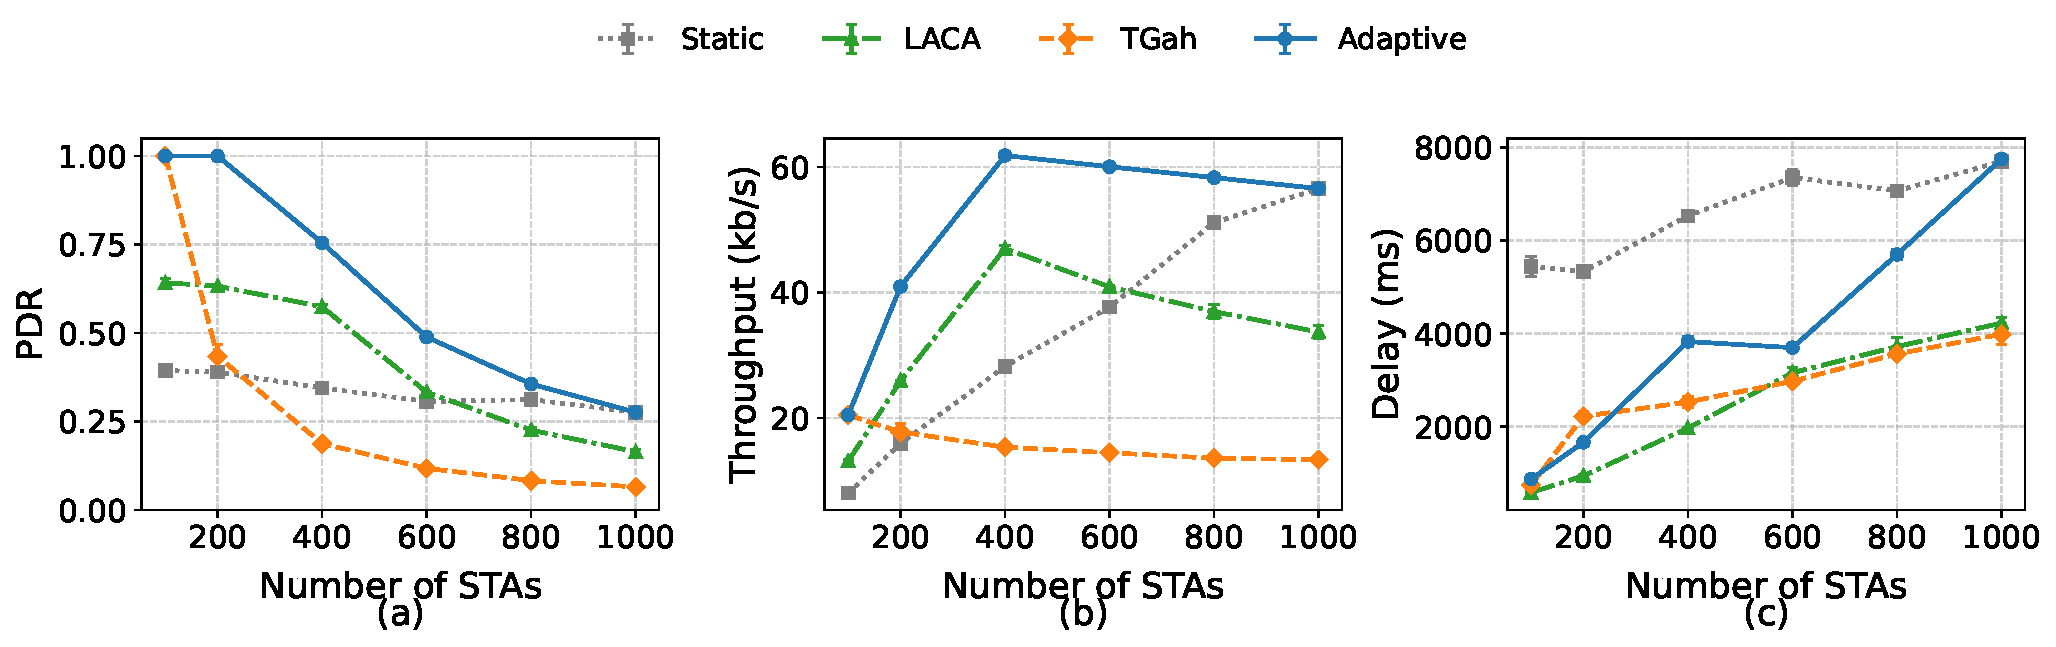
\includegraphics[width=\columnwidth]{perf_vary_n_deterministic.pdf}
	%\includegraphics[scale=0.4]{image/markov-states.pdf}
	\caption{Results obtained by varying the number of STAs under a fixed packet generation interval of 5 \textit{seconds} \rev{($0.2$ packets/s/STA)}\new{, comparing Static, LACA~\cite{10067238}, Chang2019~\cite{Chang2019TrafficAware}, and the proposed Adaptive scheme}.}
	\label{stations}
\end{figure}

Fig.~\ref{poison} presents the results under \textit{Poisson} packet arrivals \rev{with rate $\lambda_p=0.2$ packets/s/STA} and varying number of STAs, capturing the impact of stochastic and bursty traffic to study how our prediction model works. Fig.~\ref{poison}(a) shows that adaptive achieves the best PDR at every evaluated network size \new{(e.g., $0.995$ vs.\ $0.380$ (static), $0.645$ (LACA), and $0.993$ (Chang2019) at $N=100$; $0.716$ at $N=400$)}, narrowing to a near-tie with static by $N=1000$ ($0.265$ for both) as the network approaches saturation. \new{Chang2019 again starts strongest of the three baselines ($0.993$ at $N=100$) but collapses fastest ($0.063$ at $N=1000$); LACA is competitive at low $N$ but, as under deterministic traffic, drops below static once $N\ge800$ ($0.228$ vs.\ $0.300$).} The ability of the adaptive scheme to detect and respond to bursty traffic using the CUSUM--EWMA estimator enables it to allocate appropriate slot durations, thereby reducing packet losses. \new{We do not claim a specific crossover point between adaptive and static below $N=1000$ since intermediate values were not simulated.} Fig.~\ref{poison}(b) shows the throughput performance under Poisson traffic. \new{Throughput mirrors the PDR ordering: adaptive leads throughout, followed by LACA at low-to-moderate $N$, then static, with Chang2019 lowest and roughly flat ($21.3\to13.4$~kb/s) despite its early PDR advantage -- its fixed regression-based grouping fails to accommodate the burstier Poisson arrivals.} The static scheme, due to its fixed configuration, fails to efficiently accommodate traffic fluctuations, resulting in lower throughput, particularly under high load conditions. Fig.~\ref{poison}(c) illustrates the delay performance. \new{The delay of the adaptive scheme is non-monotonic with network size (e.g., $609$~ms at $N=100$ rising to $6059$~ms at $N=600$, dipping to $4931$~ms at $N=800$, and rising again to $6274$~ms at $N=1000$), reflecting the combined effect of increased contention and the larger, more variable set of delivered packets included in the delay average as PDR changes with $N$. Chang2019 maintains the lowest delay at low-to-moderate $N$ for the same reliability-driven reason as under deterministic traffic. The static scheme's delay is comparatively flatter across $N$ ($4418$--$6278$~ms), which is attributed to its lower and more stable successful transmission rate rather than more efficient scheduling; note that at $N=600$ the adaptive scheme's delay ($6059$~ms) briefly exceeds the static scheme's ($5890$~ms) despite adaptive's substantially higher PDR at that point.}

\begin{figure}[!h]
	\centering
	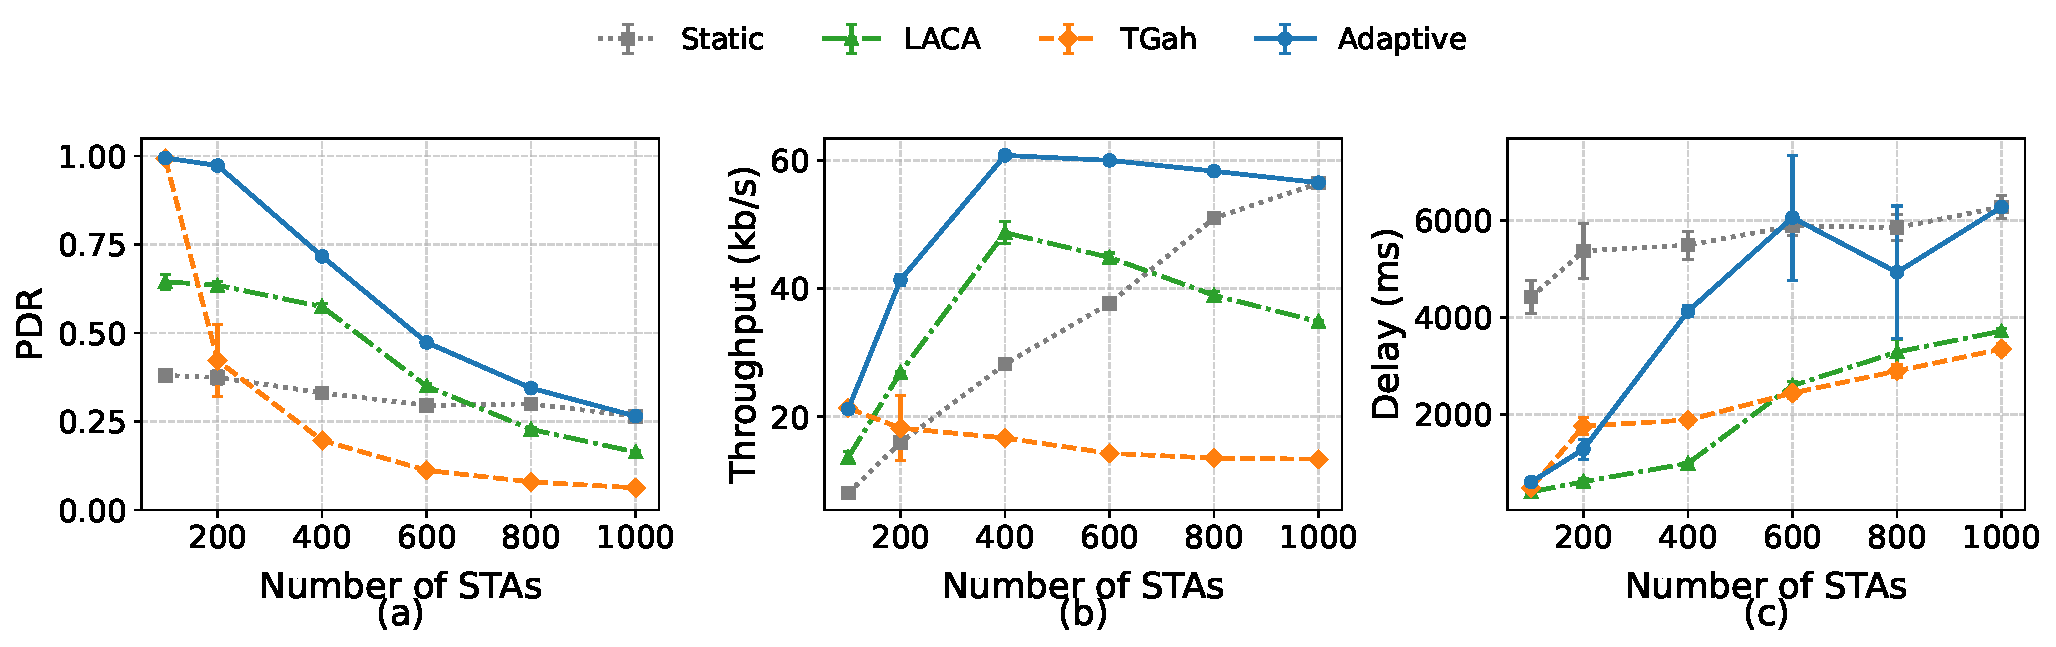
\includegraphics[width=\columnwidth]{perf_vary_n_poisson.pdf}
	\caption{Results obtained by varying the number of STAs under Poisson packet arrivals \rev{with $\lambda_p=0.2$ packets/s/STA}\new{, comparing Static, LACA, Chang2019, and the proposed Adaptive scheme}.}
	\label{poison}
\end{figure}

Fig.~\ref{packet_interval} evaluates the performance under varying packet generation intervals with the number of STAs fixed at 500. Fig.~\ref{packet_interval}(a) shows that as the packet interval increases (i.e., traffic load decreases), the PDR of all four schemes improves \new{and does so almost linearly with the interval (e.g., static PDR rises from $0.060$ at $T_p=1$~s to $0.299$ at $T_p=5$~s), with a stable ordering throughout: adaptive highest (reaching $0.595$ at $T_p=5$~s, almost exactly $2\times$ static's $0.299$), followed by LACA ($0.424$ at $T_p=5$~s), then static, with Chang2019 lowest at every interval ($0.147$ at $T_p=5$~s) -- unlike the $N$-sweeps, Chang2019 never leads here, since its group-count adaptation is tuned for scaling contention rather than light, steady load. None of the four schemes reaches near-unity reliability within this interval range at $N=500$ -- all remain contention-limited at this network size.} Fig.~\ref{packet_interval}(b) shows that \new{adaptive ($60.9$--$61.0$~kb/s), LACA ($43.4$--$45.5$~kb/s), and static ($30.6$~kb/s) all maintain an approximately \emph{constant} throughput as the packet interval increases, rather than decreasing as might be expected from the reduced offered load; only Chang2019's throughput declines slightly ($16.5\to15.1$~kb/s). This near-constant behavior for the top three schemes occurs because, at fixed $N=500$, the offered load decreases as $1/T_p$ while PDR increases approximately linearly with $T_p$ in this regime, so their product -- the delivered throughput -- remains close to constant for each scheme.} Fig.~\ref{packet_interval}(c) illustrates the delay performance. \new{Delay decreases with increasing packet interval for all four schemes due to reduced contention, following a consistent ordering at every evaluated interval: Chang2019 lowest ($4859\to2724$~ms), followed by LACA ($5772\to2744$~ms), then adaptive ($7752\to4180$~ms), with static highest throughout ($11278\to7640$~ms). Adaptive's delay exceeding LACA's despite adaptive's higher PDR reflects the same delay-vs-reliability tradeoff noted for Fig.~\ref{stations} and Fig.~\ref{poison}: adaptive delivers roughly $1.3$--$1.4\times$ as many packets as LACA at each interval (Fig.~\ref{packet_interval}(a)), and those additional delivered packets carry queuing and contention delay that LACA's lower-PDR operation excludes from its average.}

\begingroup\color{red}
To quantify STA energy consumption, we track per-node radio time in four power states (TX, RX, idle/CCA, deep sleep) and convert to energy using published power-state values for a reference sub-1~GHz IEEE~802.11ah radio (MORSE MG100: $P_{\mathrm{tx}}=180$~mW, $P_{\mathrm{rx}}=62$~mW, $P_{\mathrm{idle}}=20$~mW, $P_{\mathrm{sleep}}=0.5$~mW), consistent with published IEEE~802.11ah power-save figures~\cite{Khorov2019Tutorial}. This is a MAC-level energy accounting model driven by simulated TX/RX/idle/sleep durations rather than a chipset-measured current trace, so the reported values should be read as a comparative indicator of relative energy efficiency across policies rather than an absolute hardware energy budget.

Fig.~\ref{fig:energy} reports total energy consumption per STA. Adaptive consumes the least or near-least energy at every evaluated point except at $N=1000$ under deterministic traffic, where it converges with static ($522$ vs.\ $523$~mJ), consistent with the PDR/throughput convergence noted earlier. Chang2019 consumes by far the most energy throughout -- $1.2\times$ adaptive's consumption at $N=100$, widening to $2.2$--$2.3\times$ for $N\ge400$ (e.g., $1164$ vs.\ $522$~mJ at $N=1000$, deterministic) -- despite delivering the fewest packets, since its frequent group/slot rebalancing under high contention burns airtime on retries and collisions rather than successful delivery. LACA sits between static and Chang2019 throughout. Static's raw energy consumption is comparatively low, but -- as with its delay in Figs.~\ref{stations}--\ref{packet_interval} -- this reflects its low PDR rather than efficient operation: static simply transmits, retries, and idles less because it delivers fewer packets overall.

This last point is clearest in energy \emph{efficiency} (delivered kbit/J), which normalizes for how much useful work each joule accomplishes. Adaptive wins decisively at every evaluated point across all three sweeps: e.g., $67.6$ vs.\ $58.4$ (Chang2019), $48.2$ (LACA), and $32.6$~kbit/J (static) at $N=100$ deterministic, and $13.0$ vs.\ $1.4$, $6.1$, and $13.0$~kbit/J at $N=1000$ (adaptive ties static there, consistent with their PDR/throughput/energy convergence, while LACA and Chang2019 both fall far behind). Chang2019's efficiency collapses fastest of all four schemes as $N$ grows (from $58.4$ at $N=100$ down to $1.4$~kbit/J at $N=1000$, a $42\times$ drop), reflecting that its high raw energy consumption is spent almost entirely on unsuccessful attempts once contention exceeds what its fixed regression-based grouping can track. In the interval sweep at $N=500$, the same ordering holds at every tested interval (adaptive $\approx35.0$~kbit/J, static $\approx19.4$, LACA $\approx21.7$, Chang2019 $\approx3.8$--$4.3$~kbit/J), so adaptive is roughly $8$--$9\times$ more energy-efficient than Chang2019 and $1.6$--$1.8\times$ more efficient than static or LACA across the full swept range. Hardware-measured (as opposed to simulated) STA energy traces remain future work.

\begin{figure}[!h]
	\centering
	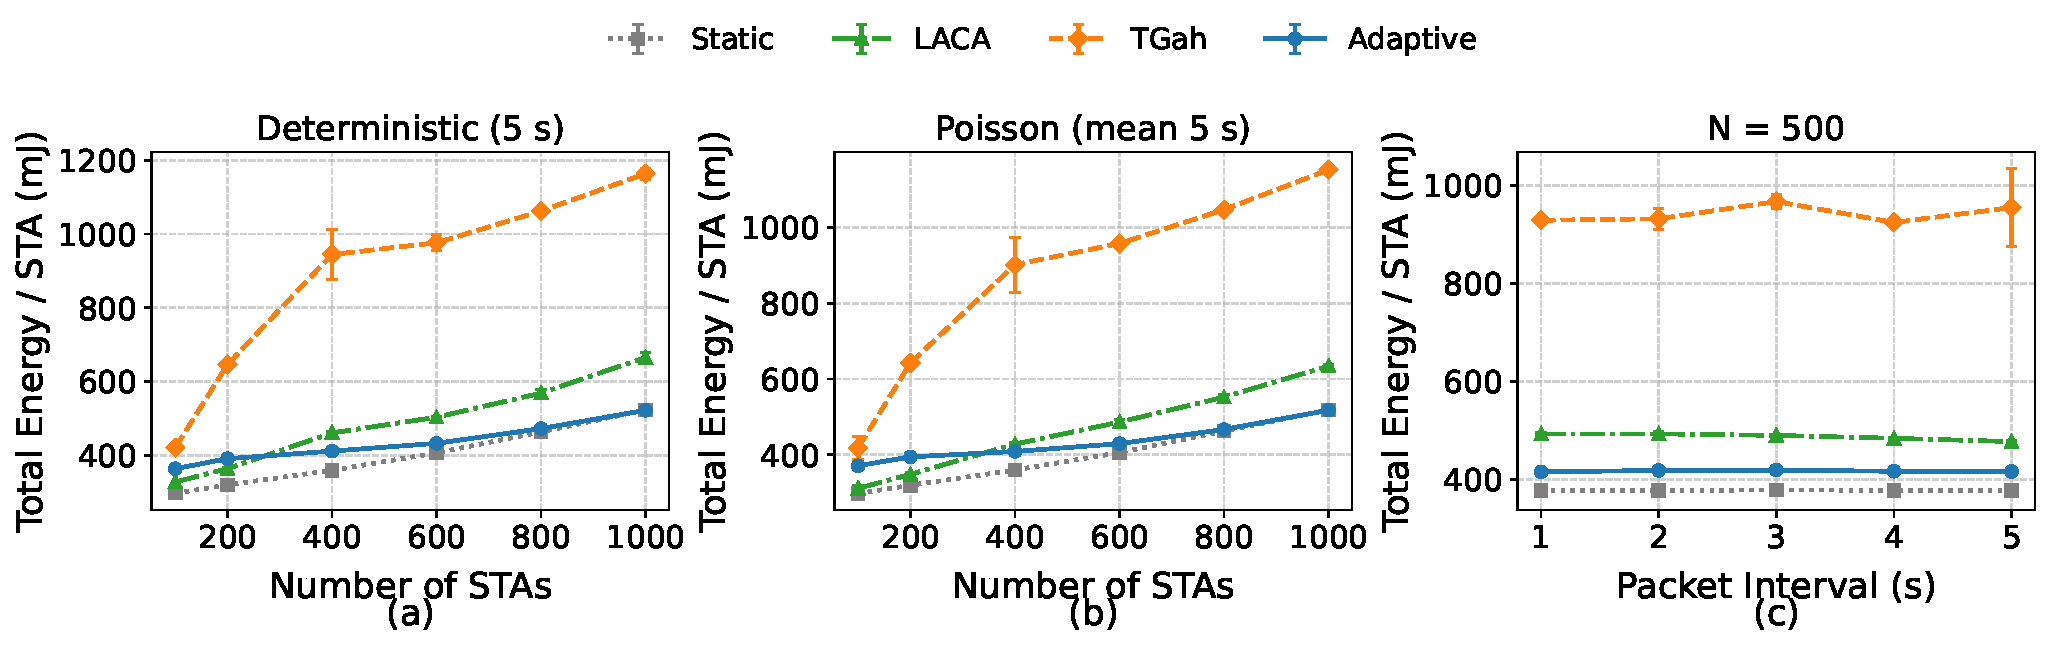
\includegraphics[width=\columnwidth]{energy_total_combined.pdf}
	\caption{Total energy consumption per STA for Static, LACA, Chang2019, and the proposed Adaptive scheme.}
	\label{fig:energy}
\end{figure}
\endgroup

\rev{The increase in throughput with the number of STAs in Figs.~\ref{stations} and~\ref{poison} should be interpreted as aggregate AP throughput, not per-STA throughput. As the number of STAs increases, the offered traffic load also increases; hence, aggregate throughput rises until the RAW configuration approaches saturation, after which the gain diminishes.} Overall, the obtained results demonstrate that the proposed adaptive RAW scheme effectively adapts to both network scale and traffic dynamics. By leveraging traffic estimation and Bianchi-based service modeling, our scheme significantly improves PDR and throughput compared to static, LACA, and Chang2019 \new{across most of the evaluated range. LACA and Chang2019 additionally underperform even the static baseline at high $N$, since neither rebalances its group/slot budget fast enough under growing contention, whereas adaptive converges specifically with static (not LACA or Chang2019) at the highest evaluated network size ($N=1000$ under deterministic traffic), which we attribute to both schemes operating near the standard-imposed RAW airtime budget under the evaluated fixed group/slot configuration ($N_g=8$, $N_s=8$).}

\begin{figure}[!h]
	\centering
	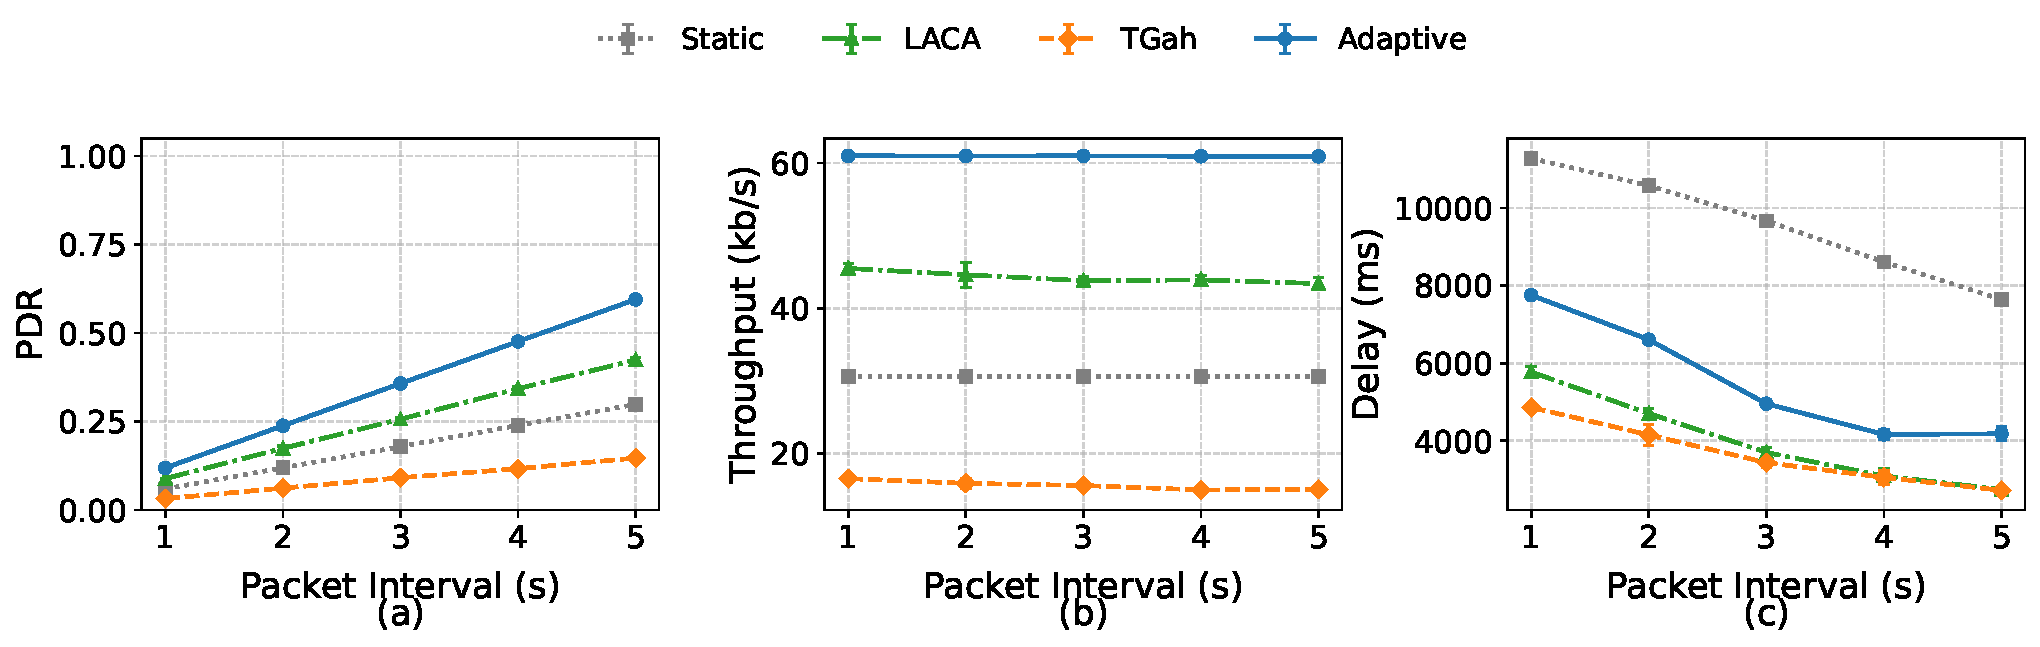
\includegraphics[width=\columnwidth]{perf_vary_interval.pdf}
	\caption{Results obtained under different packet arrivals with the number of STAs fixed at 500\new{, comparing Static, LACA, Chang2019, and the proposed Adaptive scheme}.}
	\label{packet_interval}
\end{figure}

\section{Conclusion}

This letter proposed an autonomous adaptive RAW slot sizing scheme for IEEE~802.11ah networks. By combining CUSUM--EWMA-based traffic estimation with an analytical contention model, the AP dynamically adjusts slot durations without additional signaling overhead. Results show that the proposed scheme effectively improves PDR and throughput compared to static, LACA~\cite{10067238}, and Chang2019~\cite{Chang2019TrafficAware} allocation \new{across most of the evaluated range, converging specifically with static performance at the highest evaluated network size, while LACA and Chang2019 fall behind even static under high contention}. Our proposed approach is standard-compliant and suitable for large-scale IoT networks with dynamic traffic. \rev{The present model uses Bianchi's steady-state DCF equations as a tractable contention approximation for RAW slot sizing; future work will extend the analysis to finite-horizon RAW-slot models and hardware-calibrated STA energy measurements.}


\bibliographystyle{IEEEtran}
\bibliography{refs,reviewer_added_refs}
\end{document}
